\documentclass[12pt,letterpaper]{article}
\usepackage{fontspec}
\setmainfont{Arial}
\usepackage{setspace}
\usepackage[utf8]{inputenc}
\usepackage[portuguese]{babel}
\usepackage[version=3]{mhchem}
\usepackage[journal=jacs]{chemstyle}
\usepackage{listings}
\usepackage[affil-it]{authblk} 
\usepackage{tikz}
\usepackage{hyperref}
\usepackage{cite}
\usepackage{verbatim}
\usepackage{graphicx}
\usepackage{url}     
\usepackage{amsmath} 
\usepackage{tabularx}
\usepackage{ragged2e}
\usetikzlibrary{shapes.arrows}
\usepackage{siunitx}
\sisetup{mode=text, output-decimal-marker = {,}, per-mode = symbol, qualifier-mode = phrase, qualifier-phrase = { de }, list-units = brackets, range-units = brackets, range-phrase = --}
\DeclareSIUnit[number-unit-product = \;] \atmosphere{atm}
\DeclareSIUnit[number-unit-product = \;] \pound{lb}
\DeclareSIUnit[number-unit-product = \;] \inch{"}
\DeclareSIUnit[number-unit-product = \;] \foot{ft}
\DeclareSIUnit[number-unit-product = \;] \yard{yd}
\DeclareSIUnit[number-unit-product = \;] \mile{mi}
\DeclareSIUnit[number-unit-product = \;] \pint{pt}
\DeclareSIUnit[number-unit-product = \;] \quart{qt}
\DeclareSIUnit[number-unit-product = \;] \flounce{fl-oz}
\DeclareSIUnit[number-unit-product = \;] \ounce{oz}
\DeclareSIUnit[number-unit-product = \;] \degreeFahrenheit{\SIUnitSymbolDegree F}
\DeclareSIUnit[number-unit-product = \;] \degreeRankine{\SIUnitSymbolDegree R}
\DeclareSIUnit[number-unit-product = \;] \usgallon{galón}
\DeclareSIUnit[number-unit-product = \;] \uma{uma}
\DeclareSIUnit[number-unit-product = \;] \ppm{ppm}
\DeclareSIUnit[number-unit-product = \;] \eqg{eq-g}
\DeclareSIUnit[number-unit-product = \;] \normal{\eqg\per\liter\of{solución}}
\DeclareSIUnit[number-unit-product = \;] \molal{\mole\per\kilo\gram\of{solvente}}
\usepackage{cancel}
\usepackage{graphicx}
\usepackage{lmodern}
\usepackage{fancyhdr}
\usepackage[left=4cm,right=2cm,top=3cm,bottom=3cm]{geometry}
\usepackage{titlesec}
\usepackage{enumitem}
\titleformat*{\section}{\bfseries\large}
\titleformat*{\subsection}{\bfseries\normalsize}
\usepackage{float}
\floatstyle{plaintop}
\newfloat{anexo}{thp}{anx}
\floatname{anexo}{Anexo}
\restylefloat{anexo}
\restylefloat{figure}
\usepackage[margin=10pt,labelfont=bf]{caption}
\usepackage{todonotes}
\usepackage[affil-it]{authblk} 
\usepackage{babel}
\usepackage{tikz}
\usetikzlibrary{babel}
\usepackage{siunitx}

%======================================================================

\begin{document}
\onehalfspacing 
\thispagestyle{empty}
\begin{center}
\vspace{0.2cm}

\hrulefill

UNIVERSIDADE FEDERAL DE ALAGOAS\\
PRÓ-REITORIA DE PESQUISA E PÓS-GRADUAÇÃO\\
COORDENADORIA DE PESQUISA

\hrulefill

\vspace{0.5cm}

PROGRAMA INSTITUCIONAL DE BOLSAS DE INICIAÇÃO CIENTÍFICA\\PIBIC/UFAL/FAPEAL/CNPq

\vspace{1.0cm}

\textbf{\Large{RELATÓRIO PIBIC (2017 -- 2018)}}\\

\end{center}

\vspace{1.2cm}

\textbf{TÍTULO DO PROJETO DE PESQUISA:}

\underline{Análise de Sinais e Imagens com Distâncias Estocásticas e Diferenças de Entropias}

\textbf{TÍTULO DO PLANO DE TRABALHO:}

\underline{Ferramentas para análise de séries temporais}

\vspace{1cm}

\begin{table}[!h]
\begin{center}
\begin{tabularx}{\textwidth}{|X|X|X|}
\hline                              
\textbf{Nome Orientador/Unidade/Campus/Email} &  Alejandro César Frery Orgambide/Universidade Federal de Alagoas/Campus A.C. Simões/acfrery@gmail.com\\
\hline     
\textbf{Nome Bolsista ou Colaborador} & Eduarda Tatiane Caetano Chagas\\
\hline     
\textbf{Email/Fones} & eduardachagas48@laccan.ufal.br/(82) 98858-8833\\
\hline     
\end{tabularx}
\end{center}
\end{table}

\begin{table}[!h]
\begin{center}
\begin{tabularx}{\textwidth}{|X|X|X|X|}
\hline                              
\hspace{1.3cm} X & Bolsista CNPq &  &Bolsista FAPEAL\\
\hline             
& Bolsista UFAL &  &Colaborador\\
\hline             
& Bolsista PIBIC-Af&  &\\
\hline     
\end{tabularx}
\end{center}
\end{table}

\hrulefill   

%=================================================================

\newpage
\section*{\centering \textbf{RESUMO DO PROJETO}}
\hrulefill \\

\vspace{0.8cm}

 	Este trabalho relata o processo de desenvolvimento de uma plataforma de análise dos descritores causais de uma série temporal oriundos da Teoria da Informação.
	A plataforma visa facilitar a análise dessas séries nos mais variados ramos da ciência, como por exemplo, a discriminação entre fenómenos estocásticos e caóticos~\cite{DistinguishingNoiseFromChaos}, a identificação de padrões de comportamento em redes veiculares~\cite{CharacterizationVehicleBehaviorInformationTheory},a classificação e verificação de assinaturas \textit{online}~\cite{ClassificationVerificationOnlineHandwrittenSignatures},na análise da robustez de redes~\cite{InformationTheoryPerspectiveNetworkRobustness},e a classificação de padrões de consumo de energia elétrica~\cite{CharacterizationElectricLoadInformationTheoryQuantifiers}.
 	O sistema foi implementado na linguagem de programação \texttt R que além de fornecer ferramentas gráficas, também possui uma grande precisão numérica. 
 	Ambas as características de extrema importância ao longo deste trabalho.
 Após comentar brevemente a respeito dos objetivos do projeto e a sua importância na análise não-paramétrica de séries temporais, expomos as etapas e os resultados alcançados no decorrer do projeto.\\

\textbf{Palavras-chave:} Séries Temporais, Teoria da Informação, plataforma \texttt R.

%=========================================================

\newpage
\section*{\centering \textbf{OBJETIVOS DO PROJETO DE PESQUISA}}
\hrulefill \\

Desenvolver ferramentas que visam facilitar o uso de técnicas de análise e processamento de sinais, provenientes de avanços em pesquisas voltadas a Teoria da Informação.

O estudo de séries temporais é tipicamente dividido em duas vertentes \cite{BrockwellDavis91}, a análise do domínio do tempo e do domínio da frequência, sendo utilizado em ambas abordagens os dados que resultam diretamente das observações coletadas, que por sua vez estão sujeitos a efeitos danosos de diversos tipos de contaminação. Uma solução alternativa, presente na literatura, para evitar tal contaminação consiste no uso de métodos não-paramétricos.

	O projeto objetiva facilitar a análise não-paramétrica de séries temporais, desenvolvendo um sistema de extração dos descritores causais oriundos da Teoria da Informação que auxiliam no processo de identificação do tipo de dinâmica subjacente aos dados.

%=========================================================

\newpage
\section*{\centering \textbf{OBJETIVO ESPECÍFICO DO TRABALHO DO ALUNO}}
\hrulefill \\

São objetivos específicos deste trabalho de pesquisa:

\begin{itemize}
\item Implementar funções de análise de séries temporais utilizando descritores da Teoria da Informação;
\item Implementar uma interface gráfica amigável para a aplicação de tais funções;
\item Manter a portabilidade do software para os diversos sistemas operacionais e arquiteturas de hardware;
\item Desenvolver tal projeto a partir do uso de ferramentas FLOSS (\textit{Free/Libre Open Source Software});
\item Validar a interface e as funções com usuários finais.
\end{itemize}

%=========================================================

\newpage
\section*{\centering \textbf{ETAPAS DO PLANO DE TRABALHO}}
\hrulefill \\

A metodologia de tal pesquisa consistiu em dois grandes momentos, a etapa teórica e a implementação das funcionalidades.

Para o desenvolvimento do projeto descrito neste relatório, foram planejadas as seguintes etapas de execução, que foram realizadas ao longo dos últimos meses de pesquisa.

\subsection*{Estudo das funções a serem implementadas}

O estudo das funções a serem implementadas foi realizado a partir da análise de um conjunto de referências biliográficas de qualidade, visando ampliar os conhecimentos a cerca do tema proposto.

Foram estudados ao longo deste momento, temas como séries temporais e as suas propriedades, Teoria da Informação, entropias~\cite{salicruetal1993}, distâncias estocásticas~\cite{StatisticalInferenceBasedonDivergenceMeasures} e linguagem de programação \texttt R.

\subsection*{Implementação e validação numérica}

Após o términio da revisão bibliográfica da literatura existente, foi dado então início a implementação do trabalho, desenvolvido na plataforma computacional \texttt R que além de fornecer suporte a visualização dos dados, também possui uma grande precisão numérica.

Para que tal ferramenta seja aplicada na análise de dados é de suma importância realizar a verificação de suas propriedades numéricas. Portanto, a avalição da qualidade numérica das funcionalidades desenvolvidas foi feita utilizando uma metodologia própria baseada em sistemas dinâmicos com saídas conhecidas.

\subsection*{Análise de alternativas para o desenvolvimento da interface}

Foi realizada uma pesquisa sobre as alternativas existentes para o projeto, considerando os seguintes fatores: portabilidade do software para os diversos sistemas operacionais e arquiteturas de hardware, e integração com a linguagem de programação \texttt R.

\texttt RGtk2 e \texttt Java Swing foram as alternativas iniciais para o desenvolvimento da interface gráfica. No entanto, após estudos sobre o funcionamento destas GUIs (graphical user interface), optamos pelo \texttt RGtk2, por ser uma biblioteca própria do ambiente de desenvolvimento \texttt R e pela maior facilidade em manter a portabilidade do sistema.

\subsection*{Desenvolvimento de protótipos}

Foram desenvolvidos alguns protótipos de modelos de interface com as alternativas de bibliotecas gráficas citadas anteriormente, sempre possuindo como foco a experiência com o usuário.

\subsection*{Versão de produção da interface}

Após a escolha da biblioteca \texttt RGtk2 do \texttt R, foi realizada a integração entre o ambiente gráfico e as funções de análise de séries temporais implementadas anteriormente.

\subsection*{Validação, verificação e preparação de manuais e tutoriais de uso}

Como já citado neste relatório, é de fundamental importância para tal projeto a verificação da qualidade numérica do software desenvolvido, portanto um dos seus objetivos consiste em validar a interface e as funções com usuários finais.

Até o momento da redação deste documento, os manuais e tutoriais de uso já estavam em processo de finalização, faltando apenas o processo de interação dos mesmos com o usuário.


%=========================================================

\newpage
\section*{\centering \textbf{APRESENTAÇÃO E DISCUSSÃO DOS RESULTADOS}}
\hrulefill \\

A primeira parte do projeto consistiu da apropriação do referencial teórico e análise das ferramentas disponíveis no mercado.

Há diversas ferramentas que auxiliam na análise clássica de séries temporais; para a plataforma \texttt R, existindo diversas bibliotecas para essa finalidade (ver \url{https://cran.r-project.org/web/views/TimeSeries.html}). Além destas opções, o usuário também pode contar com os softwares de visualização de séries temporais. No entanto, são limitadas as opções de bibliotecas e softwares que trabalham exclusivamente com técnicas não-paramétricas.

Apresentamos assim o desenvolvimento de uma ferramenta portável, rápida e de boa qualidade numérica que possibilita gerar novos métodos de interação do usuário com o sistema de análise, permitindo que este seja capaz de análisar os diferentes descritores oriundos da Teoria da Informação e permitir a análise gráfica dos resultados.

Seguindo o modelo de engenharia de software em espiral, o sistema foi projetado e desenvolvido de forma modular, composto pelas seguintes unidades:

\begin{itemize}
\item Módulo de simbolização;
\item Módulo de análise;
\item Modulo de visualização e interação (Em fase de desenvolvimento);
\end{itemize} 

Esses módulos foram e estão sendo desenvolvidos seguindo um cronograma. Depois passaram pelas seguintes etapas:

\begin{itemize}
\item Integração dos módulos em um sistema;
\item Teste e validação do sistema (Em fase de desenvolvimento);
\item Geração da interface gráfica (Em fase de desenvolvimento).
\end{itemize}

Permite-se a leitura de dados em vários formatos (TXT, CSV ou XLSX), e o usuário a seguir poderá escolher:

\begin{itemize}

	\item Gerar o gráfico da série (ver Figura 1);
	\item Calcular seus diversos valores de Entropia;
	\item Calcular seus diversos valores de Distâncias estocásticas;
	\item Calcular complexidades estatísticas;
    \item Identificar padrões no gráfico da série temporal;
    \item Gerar planos de Entropias;
    \item Gerar planos de Distâncias estocásticas;
	\item Gerar o histograma de padrões (ver Figura 1);
	\item Identificar o ponto característico da série no plano Entropia-Complexidade (ver Figura 1).

\end{itemize}

Um elemento original do sistema é a vinculação entre o histograma de padrões, formados através do processo de \textit{simbolização de Bandt \& Pompe}~\cite{PermutationEntropyBandtPompe}, e a série temporal. Escolhendo um ou mais elementos do histograma, os valores correspondentes na série temporal aparecem realçados. Esta funcionalidade permite a análise visual da distribuição temporal dos padrões, possibilitando futuramente a realização de outros testes.
 
 O teste e a validação do sistema são tarefas contínuas, bem como o desenvolvimento de novas funcionalidades. 
  
\begin{figure}[H]
	\centering
	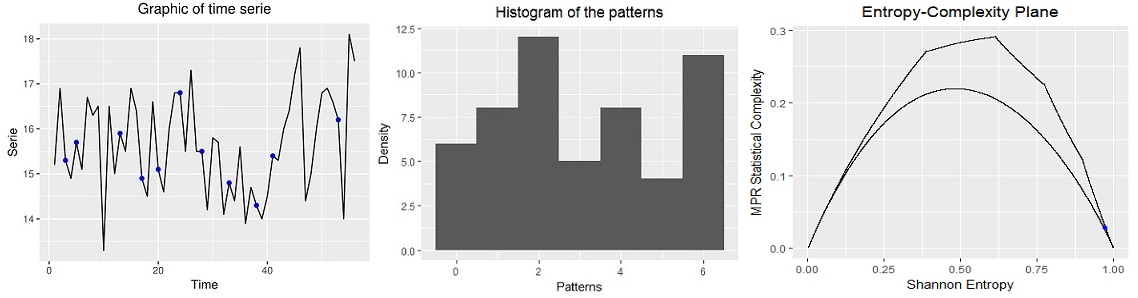
\includegraphics[width=1\columnwidth]{rplot}        
    \caption{Representação gráfica da análise de uma série temporal de produção anual de cevada por acre.}
\end{figure}
 
\begin{figure}[H]
	\centering
	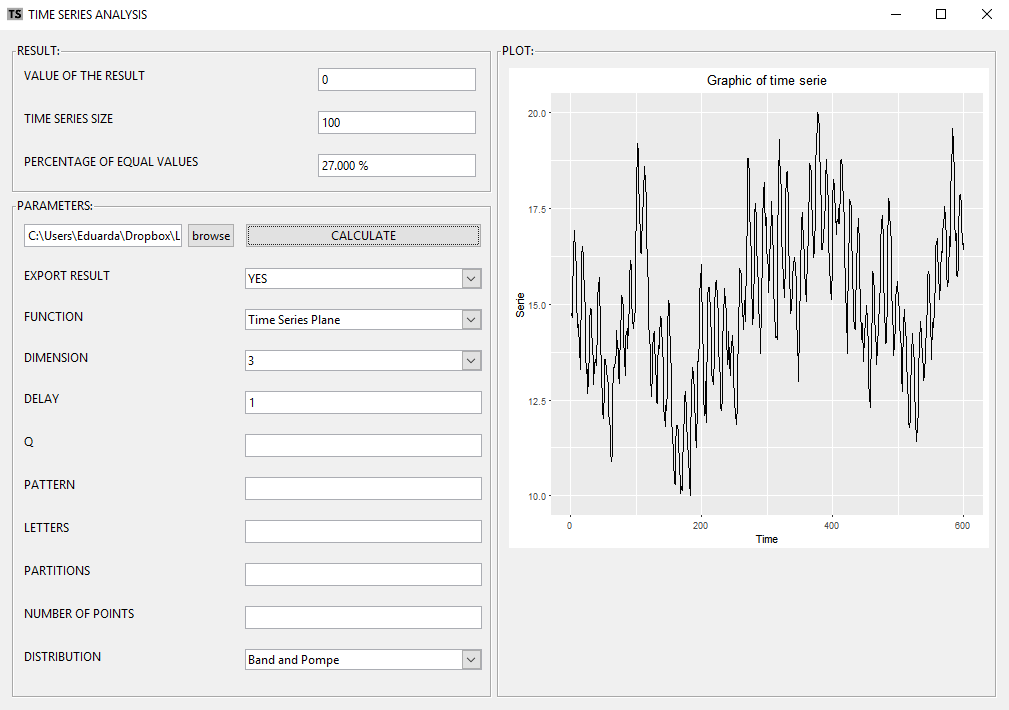
\includegraphics[width=0.95\columnwidth]{TMS}   
    \caption{Imagem atual do software em processo de desenvolvimento.}
    \vspace{6cm}
\end{figure}

%=========================================================

\newpage

\section*{\centering \textbf{CRONOGRAMA DE ATIVIDADES}}
\hrulefill \\

\textbf{Atividade 1:} Estudo das funções a serem implementadas

\textbf{Atividade 2:} Implementação e validação numérica

\textbf{Atividade 3:} Análise de alternativas para o desenvolvimento da interface

\textbf{Atividade 4:} Desenvolvimento de protótipos

\textbf{Atividade 5:} Versão de produção da interface

\textbf{Atividade 6:} Validação, verificação e preparação de manuais e tutoriais de uso


\begin{figure}[H]
	\begin{center}
		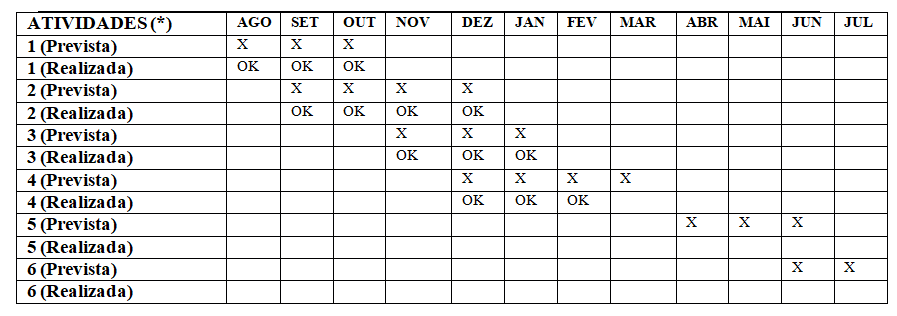
\includegraphics[width=0.95\columnwidth]{cronograma}
	\end{center}
\end{figure}

%=========================================================

\newpage

\section*{\centering \textbf{FATORES POSITIVOS E NEGATIVOS}}
\hrulefill \\

Os principais fatores positivos e negativos que interferiram na condução do projeto e plano de trabalho se encontram listados abaixo:

\section{Positivos}

\begin{itemize}
\item Aumento de conhecimento nas áreas de Estatística, Probabilidade, Análise de Dados, Teoria da Informação e Estatística Computacional;
\item Aprimoramento do conhecimento da plataforma \texttt R;
\item Experiência no desenvolvimento de software estatístico;
\item Contato com boas práticas científicas e ética profissional;
\item Participação dos seminários semanais realizados tradicionalmente pelo grupo nas dependências do LaCCAN - Laboratório de Computação Científica e Análise Numérica;
\item Oportunidade de realizar troca de conhecimento, tanto com os colegas de laboratório como com os excelentes pesquisadores que compõem o grupo.
\end{itemize}

\section{Negativos}

\begin{itemize}
\item Ausência de pacotes para a plataforma \texttt R quem realizem interação entre gráficos de forma offline.
\end{itemize}

%=====================================================================================

\newpage

\bibliographystyle{unsrt}
\bibliography{ref1}

\end{document}